\subsection{Tower reconstruction}

Our analysis used the central production of calorimeter data in which waveforms are processed using the TEMPLATE mode of the CaloWaveformProcessing module. 
For Run 2024, calorimeter towers were hardware zero suppressed with tower by tower zero suppression thresholds set by the width of each channels pedestal. 
Non zero suppressed waveforms recorded 12 time samples per event. Both EMCal and HCal templates were created using beam data from early runs of Run 2024. 
The template fit has three free parameters: the pedestal, peak time and scale of the waveform, and the processing procedure returns these parameters plus a $\chi^{2}$ term which acts as a goodness of fit metric. 
More information on the template fit method can be found in \cite{Seidlitz1}.

All three calorimeters, EMCal, IHCal and OHCal, are calibrated to the electromagnetic energy scale. 
For the EMCal, the absolute energy scale calibration is established by an $\eta$ dependent $\pi^{0}$ calibration established for groups of runs throughout Run 2024. 
More information regarding the specifics of the EMCal calibration can be found in \cite{Seidlitz1}. 
The IHCal and OHCal are both calibration to the MIP energy scale (similar to EM energy scale) using the minimum ionizing particle energy depositions from cosmic ray muons. 
Cosmics data used for the Run 2024 HCal calibrations were taken during Run 24 data taking in periods without beam. Therefore, we expect the detector conditions to be similar to beam data. More information regarding the specifics of the HCal calibration can be found in~\cite{HCal_calib_internal_note}.

\subsection{Calorimeter jet reconstruction}
Jet reconstruction was done using the anti-$k_{T}$ algorithm within the framework of the sPHENIX HIJetReco macro for R = 0.4 jets without underlying event subtraction. 
All jets are reconstructed using calorimeter towers. 
The jet reconstruction is performed using the default jet reconstruction parameters found in the \href{https://github.com/sPHENIX-Collaboration/macros/blob/master/common/HIJetReco.C}{HIJetReco.C macro} in the sPHENIX macros repo.

\subsubsection{Defining jet event geometry}
To study the underlying event in regions outside of the jet cone, the following event geometry is defined by the $\phi$ direction of the leading $\pT$ jet. 
The calorimeter acceptance is split up into three azimuthal regions with respect to the $\phi$ direction of the leading jet. 
The towards region with $\|\Delta\phi\| < 60 \degree$ from the leading jet, two transverse regions with $ 60 \degree < \|\Delta \phi\| < 120 \degree$ and an away region with $\|\Delta\phi\| > 120 \degree$. 
The towards, transverse and away regions are shown in Fig. \ref{fig:event_geometry}. 

\begin{figure}
    \centering
    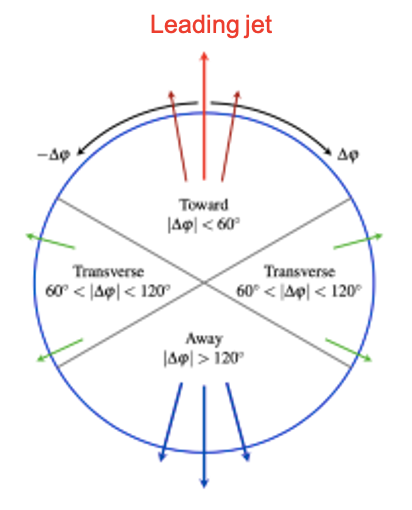
\includegraphics[width=0.3\linewidth]{Figures/event_geometry.png}
    \caption{Towards, transverse and away region definitions of jet event with respect to the leading jet azimuthal direction.}
    \label{fig:event_geometry}
\end{figure}

\subsection{Topocluster reconstruction}
Topoclusters are created using all three layers of the calorimeters. 
The default topoclustering parameters found in the \href{https://github.com/sPHENIX-Collaboration/macros/blob/master/common/G4_TopoClusterReco.C}{G4\_TopoClusterReco.C macro} in the sPHENIX macros repo are as follows: 
\begin{verbatim}
  RawClusterBuilderTopo* ClusterBuilder = new 
            RawClusterBuilderTopo("HcalRawClusterBuilderTopo");
  ClusterBuilder->Verbosity(verbosity);
  ClusterBuilder->set_nodename("TOPOCLUSTER_ALLCALO");
  ClusterBuilder->set_enable_HCal(true);
  ClusterBuilder->set_enable_EMCal(true);
  ClusterBuilder->set_noise(IHCal_noise, OHCal_noise, EMCal_noise);
  ClusterBuilder->set_significance(4.0, 2.0, 0.0);
  ClusterBuilder->allow_corner_neighbor(true);
  ClusterBuilder->set_do_split(true);
  ClusterBuilder->set_minE_local_max(1.0, 2.0, 0.5);
  ClusterBuilder->set_R_shower(0.025);
  ClusterBuilder->set_use_only_good_towers(true);
  ClusterBuilder->set_absE(true);
  se->registerSubsystem(ClusterBuilder);  
\end{verbatim}

\subsubsection{Setting topocluster noise thresholds}
For this analysis, we need to optimize the topocluster noise thresholds for the state of the calorimeter noise during the full Run 2024 p+p running.
The first step of this process is to find the tower-by-tower pedestal RMS for each calorimeter layer from pedestal data (Run 54256). These tower-by-tower pedestal RMS values are shown in Figure~\ref{fig:pedestal_RMS}. The means of these tower-by-tower pedestal RMS are extracted for each of the calorimeters from these plots. The EMCal mean RMS = 30.4 MeV, the IHCal mean RMS = 1.77 MeV, and the OHCal mean RMS = 11.7 MeV.

From previous studies of changes in the calorimeter noise across the p+p running done by the calorimeter calibrations group, it is known that the EMCal noise increased across the p+p running while the IHCal and OHCal noise stayed fairly constant. Therefore, the pedestal data in Run 54256 (taken after the p+p running period, just before Au+Au running) is an overestimate of the EMCal average noise across the full 0 + 1.5 mrad running period. In the nominal simulation production a scaling factor of 0.75 is applied to the pedestal noise fluctuations so that the simulation matches the pedestal region of beam runs from 0 + 1.5mrad p+p data. This same scaling factor of 0.75 is applied to the EMCal mean RMS for consistency giving a EMCal mean RMS of 22.8 MeV for pedestal fluctuations during the 2024 p+p running. 

Now with accurate values for the pedestal effects in each of the calorimeters during the 2024 p+p running, the truth particle to topocluster matching is tested for two, three and four times the mean pedestal RMS values of the calorimeter layer using the Run 22 minbias simulation sample with realistic pedestal noise embedded. The topocluster sensitivity to noise is tested by finding the relative width of the E/p distributions for topoclusters matched to truth particles. More details on this method are included in the next section, Section~\ref{sec:topo_resolution}. 
The full set of tested pedestal RMS values are included in Table~\ref{tab:topo_noise_parameters}. 
\begin{table}[]
    \centering
    \begin{tabular}{c|c|c|c|c|c}
        Calorimeter & Run 54256 $\langle \sigma_{ped} \rangle$ & p+p running $\langle \sigma_{ped} \rangle$ & p+p $\langle 2\sigma_{ped} \rangle$ & p+p $\langle 3\sigma_{ped} \rangle$ & p+p $\langle 4\sigma_{ped} \rangle$ \\
        \hline
        EMCal & 30.4 & 22.8 & 45.6 & 68.4 & 91.2 \\
        IHCal & 1.77 & 1.77 & 3.5 & 5.3 & 7.0 \\
        OHCal & 11.7 & 11.7 & 23.4 & 35.1 & 46.8 \\
    \end{tabular}
    \caption{Table of pedestal RMS values extracted and used as topocluster noise parameters for p+p running. All $\sigma_{ped}$ values are given in MeV.}
    \label{tab:topo_noise_parameters}
\end{table}

\begin{figure}
    \centering
    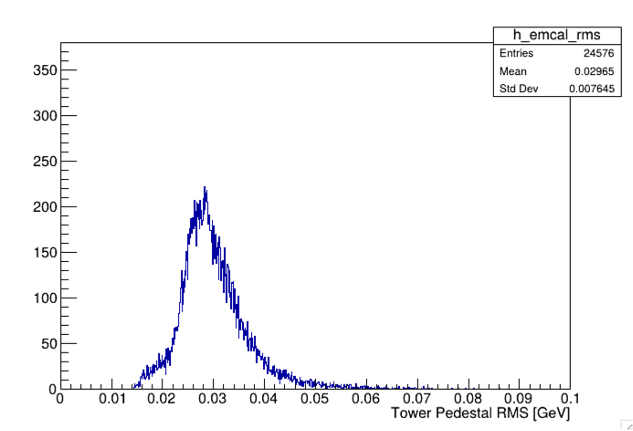
\includegraphics[width=0.32\linewidth]{Figures/topocluster_noise/emcal_pedestal_rms.png}
    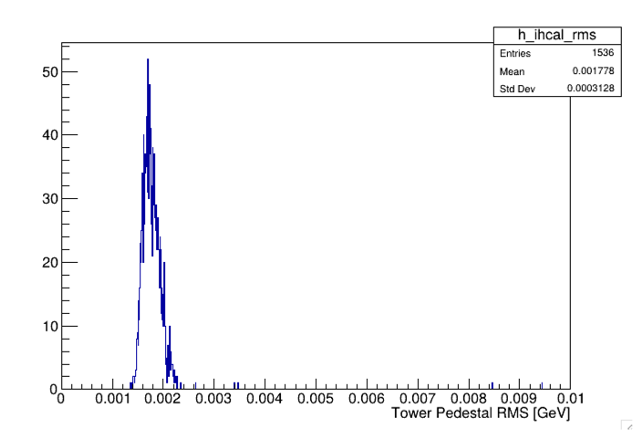
\includegraphics[width=0.32\linewidth]{Figures/topocluster_noise/ihcal_pedestal_rms.png}
    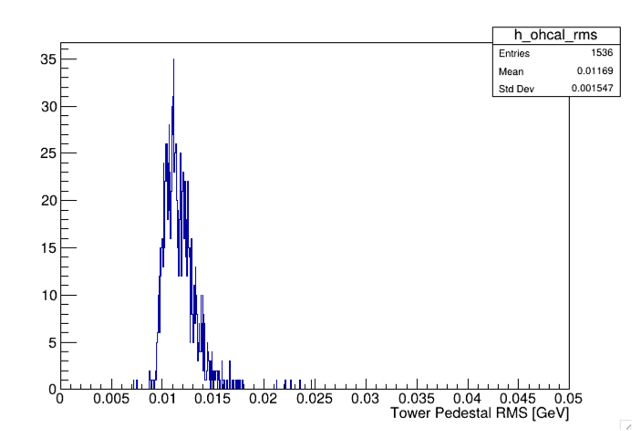
\includegraphics[width=0.32\linewidth]{Figures/topocluster_noise/ohcal_pedestal_rms.png}
    \caption{Tower-by-tower pedestal RMS for EMCal (left), IHCal (middle) and OHCal (right) found from pedestal run 54256. Mean RMS is extracted, scaled to match pedestal in beam data and used for testing noise thresholds in topocluster seeding.}
    \label{fig:pedestal_RMS}
\end{figure}

\subsubsection{Resolution of Topoclusters}
\label{sec:topo_resolution}

The resolution of topoclusters is studied separately for electromagnetic (EM) and hadronic particles, using two distance thresholds for truth particle-topocluster matching: $\Delta R < 0.1$ and $\Delta R < 0.2$. 
To ensure the quality of the matched truth–reconstructed pairs, specific selection criteria are applied. An isolation condition is enforced, requiring the truth particle to have no other nearby truth particles with transverse momentum $p_T > 0.2$\,GeV within a cone of $\Delta R < 0.6$. 
Additionally, this study of the topocluster resolution only used events within $|z| < 30$ cm as originally the analysis was planned to use events within $|z| < 30$ cm. 

The analysis is performed for the three noise suppression thresholds: $\langle2\sigma_{ped}\rangle$, $\langle3\sigma_{ped}\rangle$, and $\langle4\sigma_{ped}\rangle$. The explicit values for these noise threshold are given in Table~\ref{tab:topo_noise_parameters} and the methodology for determining this values is outlined in the above section. These thresholds are used to evaluate how noise impacts the resolution performance of topoclusters.

For EM particles, the properties of the closest matched topocluster are examined. 
Only clusters with energy $E > 1$\,GeV are included. 
The resolution is quantified using the $E/P$ ratio, where $E$ is the energy of the matched cluster and $P$ is the momentum of the corresponding truth particle. 
Figure~\ref{fig:ep_resolution} shows the $E/P$ distributions for different noise thresholds at $\Delta R < 0.1$ for electromagnetic particles. 
The extracted resolutions from these distributions are 13.7\%, 13.4\%, and 13.3\% for the $\langle2\sigma_{ped}\rangle$, $\langle3\sigma_{ped}\rangle$, and $\langle4\sigma_{ped}\rangle$ thresholds, respectively. 
These values are consistent with results obtained from test beam measurements. 

\begin{figure}[H]
  \centering
  \begin{subfigure}[b]{0.31\textwidth}
    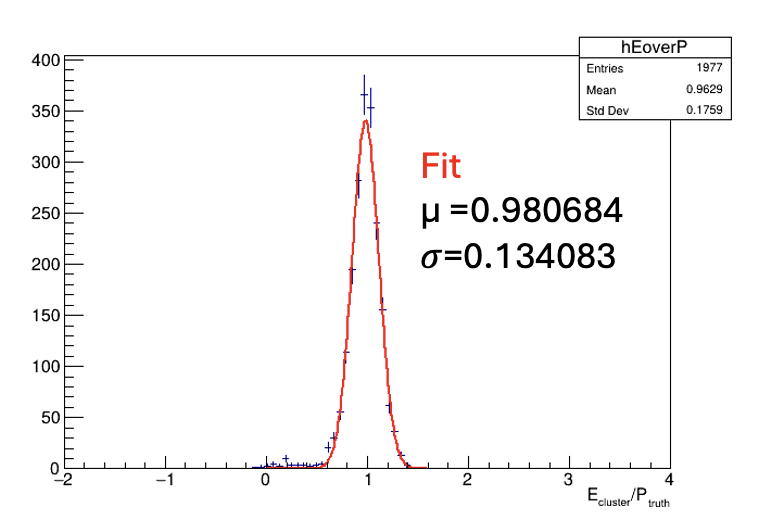
\includegraphics[width=\textwidth]{Figures/topocluster_noise/Resolution_topocluster/ep_2sigma.png}
    \caption{$2\sigma$}
  \end{subfigure}
  \hfill
  \begin{subfigure}[b]{0.32\textwidth}
    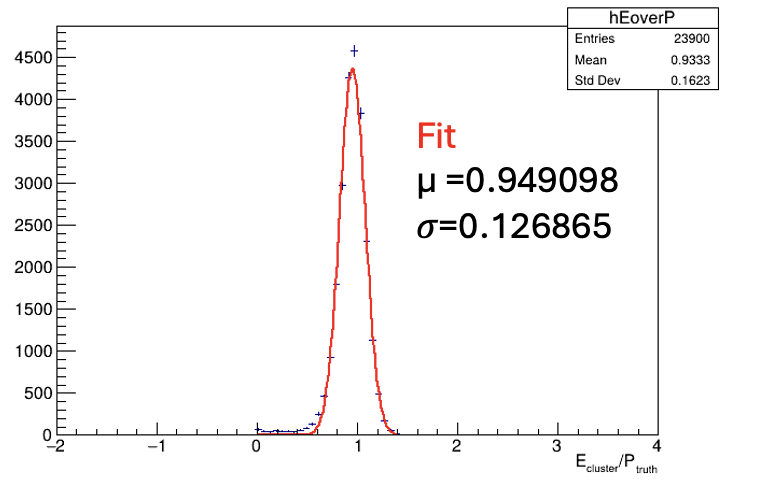
\includegraphics[width=\textwidth]{Figures/topocluster_noise/Resolution_topocluster/ep_3sigma.png}
    \caption{$3\sigma$}
  \end{subfigure}
  \hfill
  \begin{subfigure}[b]{0.31\textwidth}
    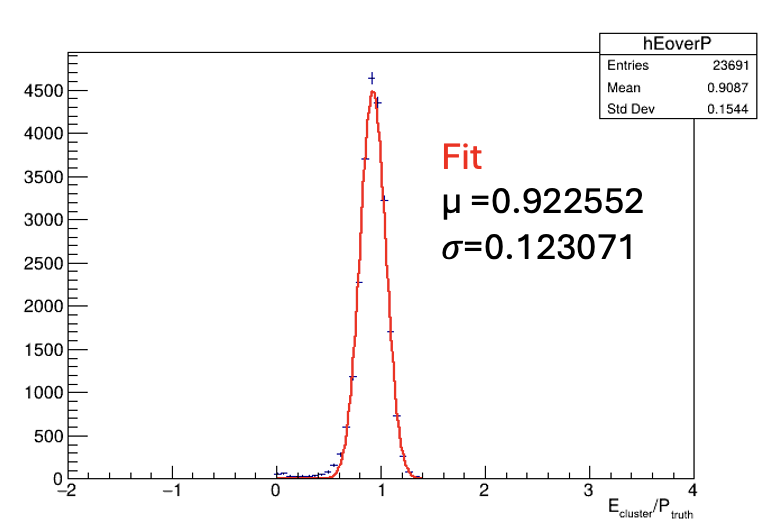
\includegraphics[width=\textwidth]{Figures/topocluster_noise/Resolution_topocluster/ep_4sigma.png}
    \caption{$4\sigma$}
  \end{subfigure}
  \caption{$E/P$ distributions for electromagnetic particles at $\Delta R < 0.1$ for different noise thresholds.}
  \label{fig:ep_resolution}
\end{figure}

\begin{figure}[H]
  \centering
  \begin{subfigure}[b]{0.32\textwidth}
    \centering
    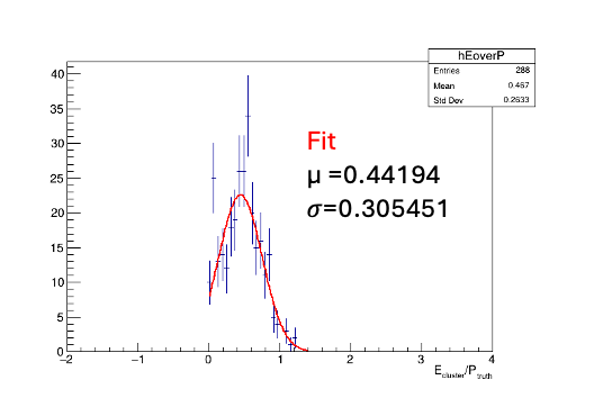
\includegraphics[width=\textwidth]{Figures/topocluster_noise/Resolution_topocluster/ep_hadronic_2sigma_e3gev_dr02.png}
    \caption{$2\sigma$}
  \end{subfigure}
  \hfill
  \begin{subfigure}[b]{0.32\textwidth}
    \centering
    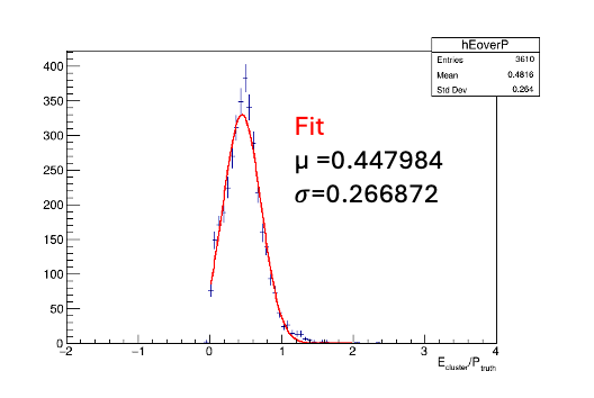
\includegraphics[width=\textwidth]{Figures/topocluster_noise/Resolution_topocluster/ep_hadronic_3sigma_e3gev_dr02.png}
    \caption{$3\sigma$}
  \end{subfigure}
  \hfill
  \begin{subfigure}[b]{0.32\textwidth}
    \centering
    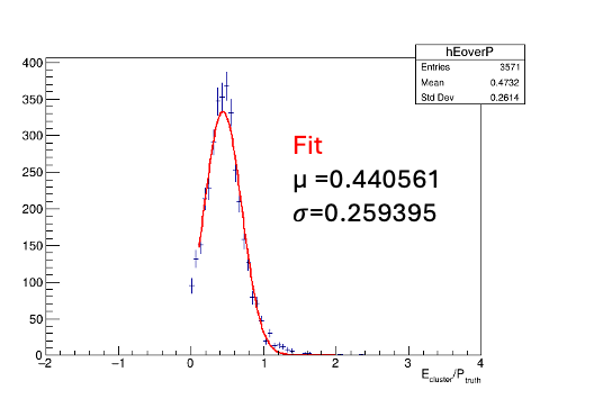
\includegraphics[width=\textwidth]{Figures/topocluster_noise/Resolution_topocluster/ep_hadronic_4sigma_e3gev_dr02.png}
    \caption{$4\sigma$}
  \end{subfigure}
  \caption{$E/P$ distributions for hadronic particles with $E > 3$\,GeV at $\Delta R < 0.2$ for different noise thresholds.}
  \label{fig:ep_hadronic_dr02_e3gev}
\end{figure}

The $E/P$ distributions for hadronic particles with $E > 3$\,GeV and matched within $\Delta R < 0.2$ are shown in Fig.~\ref{fig:ep_hadronic_dr02_e3gev} for the $\langle2\sigma_{ped}\rangle$, $\langle3\sigma_{ped}\rangle$, and $\langle4\sigma_{ped}\rangle$ noise thresholds.
The extracted resolutions for hadronic particles under these conditions are found to be 69.1\%, 59.6\%, and 58.9\% for the $\langle2\sigma_{ped}\rangle$, $\langle3\sigma_{ped}\rangle$, and $\langle4\sigma_{ped}\rangle$ thresholds, respectively.  
The resolutions obtained with the $\langle3\sigma_{ped}\rangle$ and $\langle4\sigma_{ped}\rangle$ thresholds are significantly better and are found to be very similar to each other in most cases. 
Based on this observation, the $\langle3\sigma_{ped}\rangle$ threshold is selected as the optimal working point, balancing resolution performance and noise suppression.

Additional studies were performed for hadronic particles with $E < 1$ GeV and matched within $\Delta R < 0.2$.
However for lower energy particles, the magnetic field effects become more significant and the matching between truth particles and topoclusters becomes more difficult.
A short study was performed studying the resolution of hadronic particles with $E < 1$ GeV and matched within $\Delta R < 0.2$ to tracks and the track projection module was used to match these tracks to the topoclusters.
The results of this study showed that the resolution of hadronic particles with $E < 1$ GeV and matched within $\Delta R < 0.2$ to tracks was not significantly better than the resolution of hadronic particles with $E > 3$ GeV and matched within $\Delta R < 0.2$.
These lower energy hadron simulation studies are included in Appendix~\ref{sec:additional_topo_reso}.

\subsection{Reconstructed UE Energy from towers versus topoclusters}
The reconstructed transverse energy in dijet events from summing calorimeter towers versus summing topoclusters are shown in Figure~\ref{fig:towers_and_topo} with the $\langle3\sigma_{ped}\rangle$ noise thresholds for the topocluster seeding. 
The \ET{} distribution from towers is wider than the distribution from topoclusters.
Notably, the mean topocluster \ET{} in the transverse region is about half the tower sum \ET{} in the transverse region, meaning likely the towers measurement contains a large noise contribution. 
Previous initial studies of this analysis presented in the jet group meeting also found the reconstructed \ET{} to be highly dependent on the reconstruction method and noise contributions while the \ET{} from topoclusters is much less dependent on the reconstruction method and noise level. The current final state of this analysis uses the default calorimeter calibration and reconstruction. However, details on these initial studies of the calorimeter reconstruction effects on the measurement are included in Appendix~\ref{sec:initial_studies}.
This information combined with the robustness of the topoclusters to noise and calorimeter reconstruction makes using the topoclusters with optimized noise thresholds, the best choice for this measurement. 

\begin{figure}
    \centering
    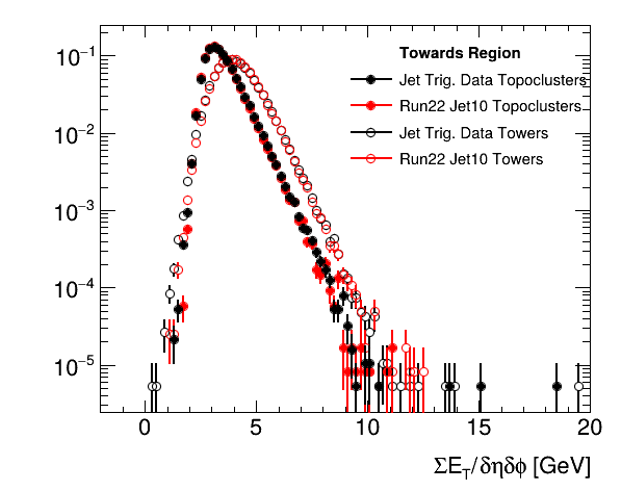
\includegraphics[width=0.32\linewidth]{Figures/topocluster_noise/towards_ET.png}
    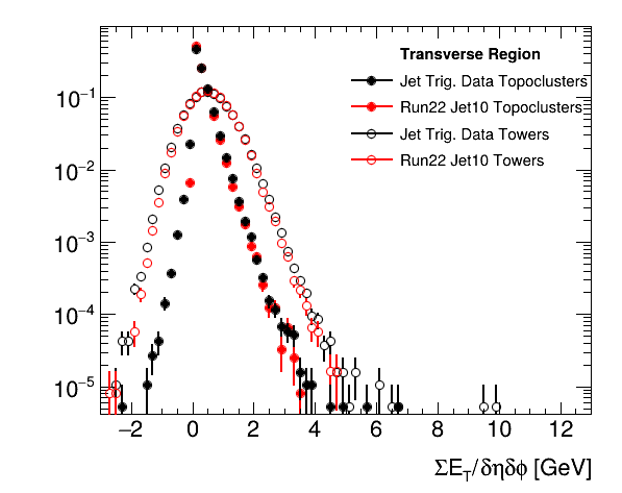
\includegraphics[width=0.32\linewidth]{Figures/topocluster_noise/transverse_ET.png}
    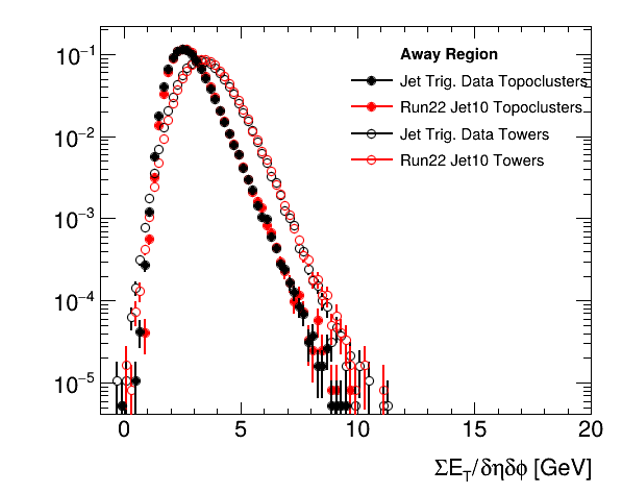
\includegraphics[width=0.32\linewidth]{Figures/topocluster_noise/away_ET.png}
    \caption{Comparison of towards, transverse and away region energy distributions from topoclusters (solid points) and towers (hollow points) in dijet events using ana468p012\_v001 data (black) and Run 22 Jet 10 simulation (red) datasets.}
    \label{fig:towers_and_topo}
\end{figure}